\documentclass{exam}

\usepackage{amsmath,amssymb,amsfonts,amsthm,dsfont}
\usepackage{lib/extra}
\usepackage{graphicx}
\usepackage{tikz}
\usepackage{enumitem}
\usepackage{float}
\usepackage{bbm}

\title{MTH 464 HW 1}
\author{Brandyn Tucknott}
\date{15 January 2025}

\begin{document}
\maketitle

\begin{questions}
    \question
A fair coin is tossed. If the coin results in a head, Die 1 with faces 1 through 6 is rolled and the up face is recorded. If the coin results in a tails, Die 2 with one face with value 1, 2 faces with value 2, and three faces with value 3 is rolled and the up face recorded. The dice are such that each face can be a top face with probability $\frac{1}{6}$. The process is repeated, with $X_j$ denoting the value of the rolled die's top face in the $j^{th}$ iteration.

\begin{parts}
    \part
    Find $P(X_1 = 3)$
    \sol
    $$P(X_1 = 3) = P(\text{3 on Die 1})P(\text{Die 1}) + P(\text{3 on Die 2})P(\text{Die 2}) = \frac{1}{6}\cdot\frac{1}{2} + \frac{1}{2}\cdot\frac{1}{2} = \frac{1}{3}$$
    
    \part
    Let $Y$ denote the number of iterations needed until the first time the value of the rolled die's top face is 3. Find $P(Y = k)$.
    \sol
    Note that $X$ is exchangeable, i.e. $P(X_j = k) = P(X_1 = k)$. Using this observation allows us to compute the following:
    $$P(Y = k) = P(\text{3 on }k^{th} \text{ roll}) + P(\text{no 3 on all $k - 1$ rolls}) =$$

    $$P(3 \text{ on the first roll}) + \paren{1 - P(3 \text{ on the first roll})}^{k - 1} = \frac{1}{3} \cdot \paren{\frac{2}{3}}^{k - 1}$$
\end{parts}

\newpage
\question
A bank classifies customers as having good or bad credit risks. Based on historical data, the bank observes that 1\% of customers with good credit record and 10\% of customers with bad credit record overdraft in their accounts in a given month. That is, with $O$ denoting the event of overdraft in a month, and $G, B$ denoting the events of good or bad credit record respectively, we have that $P(O | G) = 0.01, P(O | B) = 0.1$.
\newline
A new customer, which the bank assigns a 70\% chance of having a good credit risks, overdrafts in the first month. Find $P(G | O)$.
\sol
$$P(O) = P(O | G)P(G) + P(O | B)P(B) = (0.01)(0.7) + (0.1)(0.3) = 0.007 + 0.03 = 0.037$$
$$P(G | O) = \frac{P(O | G)P(G)}{P(O)} = \frac{(0.01)(0.7)}{0.037} = 0.189$$

\newpage
\question
A random walker starts at 0 on the $x-$axis and at each time unit steps 1 unit to the left or right, each with probability $\frac{1}{2}$. Using the normal approximation to a binomial, estimate the probability that after 100 steps, the walker is more than 10 units away from his starting position. Express your answer as an integral of the pdf of a normal random variable over the appropriate interval and use the table of values provided to approximate its value.
\sol
Define $X\sim \text{Bern}\paren{\frac{1}{2}}$, and $Y = 2X - 1$. Observe that when $X = 0, Y = -1$, and when $X = 1, Y = 1$. Then our random walk is equivalent to $S = \sum_{j = 1}^{100} Y_j$. We now calculate the mean and variance in order to use the DeMoivre-Laplace Central Limit Theorem.

$$E(Y) = E(2X - 1) = 2(\frac{1}{2}) - 1 = 0$$
$$\text{Var}(Y) = \text{Var}(2X - 1) = 4(\frac{1}{4}) = 1$$

Using these, we can find the mean and variance of our random walk where $n = 100$ steps:
$$\mu = nE(Y) = 100 \cdot 0 = 0$$
$$\sigma^2 = n\text{Var}(Y) = 100\cdot 1 = 100$$

Then by DeMoivre-Laplace, $S \sim N(0, 100)$. We wish to find the probability $P(|S| > 10)$. Before we normalize the distribution, we need the z-score of S. This is easily calculated to be $Z = \frac{S - \mu}{\sigma} = \frac{S}{10}$

$$P(|S| > 10) = P\paren{\abs{\frac{S}{10}} > 1} = P(|Z| > 1) = 2P(Z > 1) = 2\paren{1 - P(Z \leq 1)}$$

For continuity correction, we add $\frac{0.5}{10} = 0.05$ to the RHS of the inequality, giving us
$$P(|S| > 10) = 2P(1 - P(|Z| \leq 1.05))$$

This is easily evaluated to
$$2(1 - P(|Z| \leq 1.05)) = 2P(1 - 0.8531) = 0.2938$$
using a standard normal table, and we conclude that the probability of ending more than 10 units away after the random walk is 0.2938.


\newpage
\question
For $(x,y) \in \R^2$, define
$$f(x, y) =
\begin{cases}
    \frac{1}{x}, & 0 < y < x < 1 \\
    0, & \text{otherwise} \\
\end{cases}$$

\begin{parts}
    \part % part a
    Show that $f$ is a probability density function.
    \sol
    We must verify that $\iint_D f(x, y)dA = 1$.
    $$\iint_D f(x, y)dA = \int_0^1 \int_0^x \frac{1}{x} dydx = \int_0^1 1 dx = 1$$

    \part % part b
    Assume that $f$ is the joint probability density function for random variables $X, Y$. Find the marginal densities $f_X(x)$ and $f_Y(y)$.
    \sol
    $$f_X(x) = \int_0^x \frac{1}{x}dy = 1 \cdot \mathbbm{1}_{(0, 1)}(x)$$

    $$f_Y(y) = \int_y^1 \frac{1}{x}dx = -\ln y \cdot \mathbbm{1}_{(0, 1)}(y)$$

    \part % part c
    Find $E(X)$ and $E(Y)$.
    \sol
    $$E(X) = \npint xf_X(x)dx = \int_0^1 xdx = \frac{1}{2}$$

    $$E(Y) = \npint yf_Y(y)dy = \int_0^1 -y\ln y dy = \frac{1}{4}$$

    \part % part d
    Are $X, Y$ independent? Justify your answer.
    \sol
    $X, Y$ are not independent since $\frac{1}{x} \neq 1 \cdot -\ln y \longrightarrow f(x, y) \neq f_X(x)f_Y(y)$

    \part % part e
    What is the conditional density of $Y$ given $X = x$?
    \sol
    $$f_{Y | X}(y | x) = \frac{f(x, y)}{f_X(x)} = \frac{\frac{1}{x}}{1} = \frac{1}{x} \cdot \mathbbm{1}_{(0, x)}(y)$$
\end{parts}

\newpage
\question
Assume $X$ is an exponential random variable with parameter 1 and that $Y$ is an exponential random variable with parameter 2. Assume further that $X, Y$ are independent.

\begin{parts}
    \part
    Find $P(X > Y)$.
    \sol
    Our domain $D$ is such that $0 < y < x < \infty$, and we recognize that the joint pdf of $X, Y$ is 
    $$f_{X, Y}(x, y) = f_X(x)f_Y(y) = e^{-x} 2e^{-2y} \text{. To find $P(X > Y)$, we integrate the joint pdf over the domain}$$
    $$\iint_D f_{X, Y}(x, y)dA = \zpint \int_0^x e^{-x} 2e^{-2y} dydx = \zpint e^{-x}\paren{1 -e^{-2x}}dx = \zpint e^{-x}dx - \zpint e^{-3x}dx = \frac{2}{3}$$

    We conclude that the probability $P(X > Y) = \frac{2}{3}$

    \part
    Determine $a$ such that $P(X > aY) = \frac{1}{2}$
    \sol
    Define our domain $D$ is such that $0 < ay < x < \infty$, and note the joint pdf of $X, Y$ is 
    $$f_{X, Y}(x, y) = f_X(x)f_Y(y) = e^{-x} 2e^{-2y} \text{. To find $P(X > aY)$, we integrate the joint pdf over the domain}$$
    $$\iint_D f_{X, Y}(x, y)dA = \zpint \int_0^{\frac{x}{a}} e^{-x} 2e^{-2y} dydx = \zpint e^{-x}\paren{1 -e^{-\frac{2x}{a}}}dx = \zpint e^{-x}dx - \zpint e^{-\paren{\frac{2}{a} + 1}x}dx = 1 - \frac{1}{\frac{2}{a} + 1}$$

    We now set the equation to $\frac{1}{2}$ and solve for $a$.
    $$P(X > aY) = 1 - \frac{1}{\frac{2}{a} + 1} = \frac{1}{2}$$
    $$\frac{1}{\frac{2}{a} + 1} = \frac{1}{2} \longrightarrow a = 2$$

    We conclude that $P(X > aY) = \frac{1}{2}$ when $a = 2$.
\end{parts}

\newpage
\question
Assume $U, V$ are independent random variables uniformly distributed on the interval $[0, 1]$. Let $W = U + V$ and denote by $f_W(w)$ its density. Identify the correct graph for $f_W(w)$ and give a brief explanation for what is incorrect about the others.

\begin{figure}[H] % [H] exact placement
\vspace{-1.4in} % move the figures up closer to the question
\centering
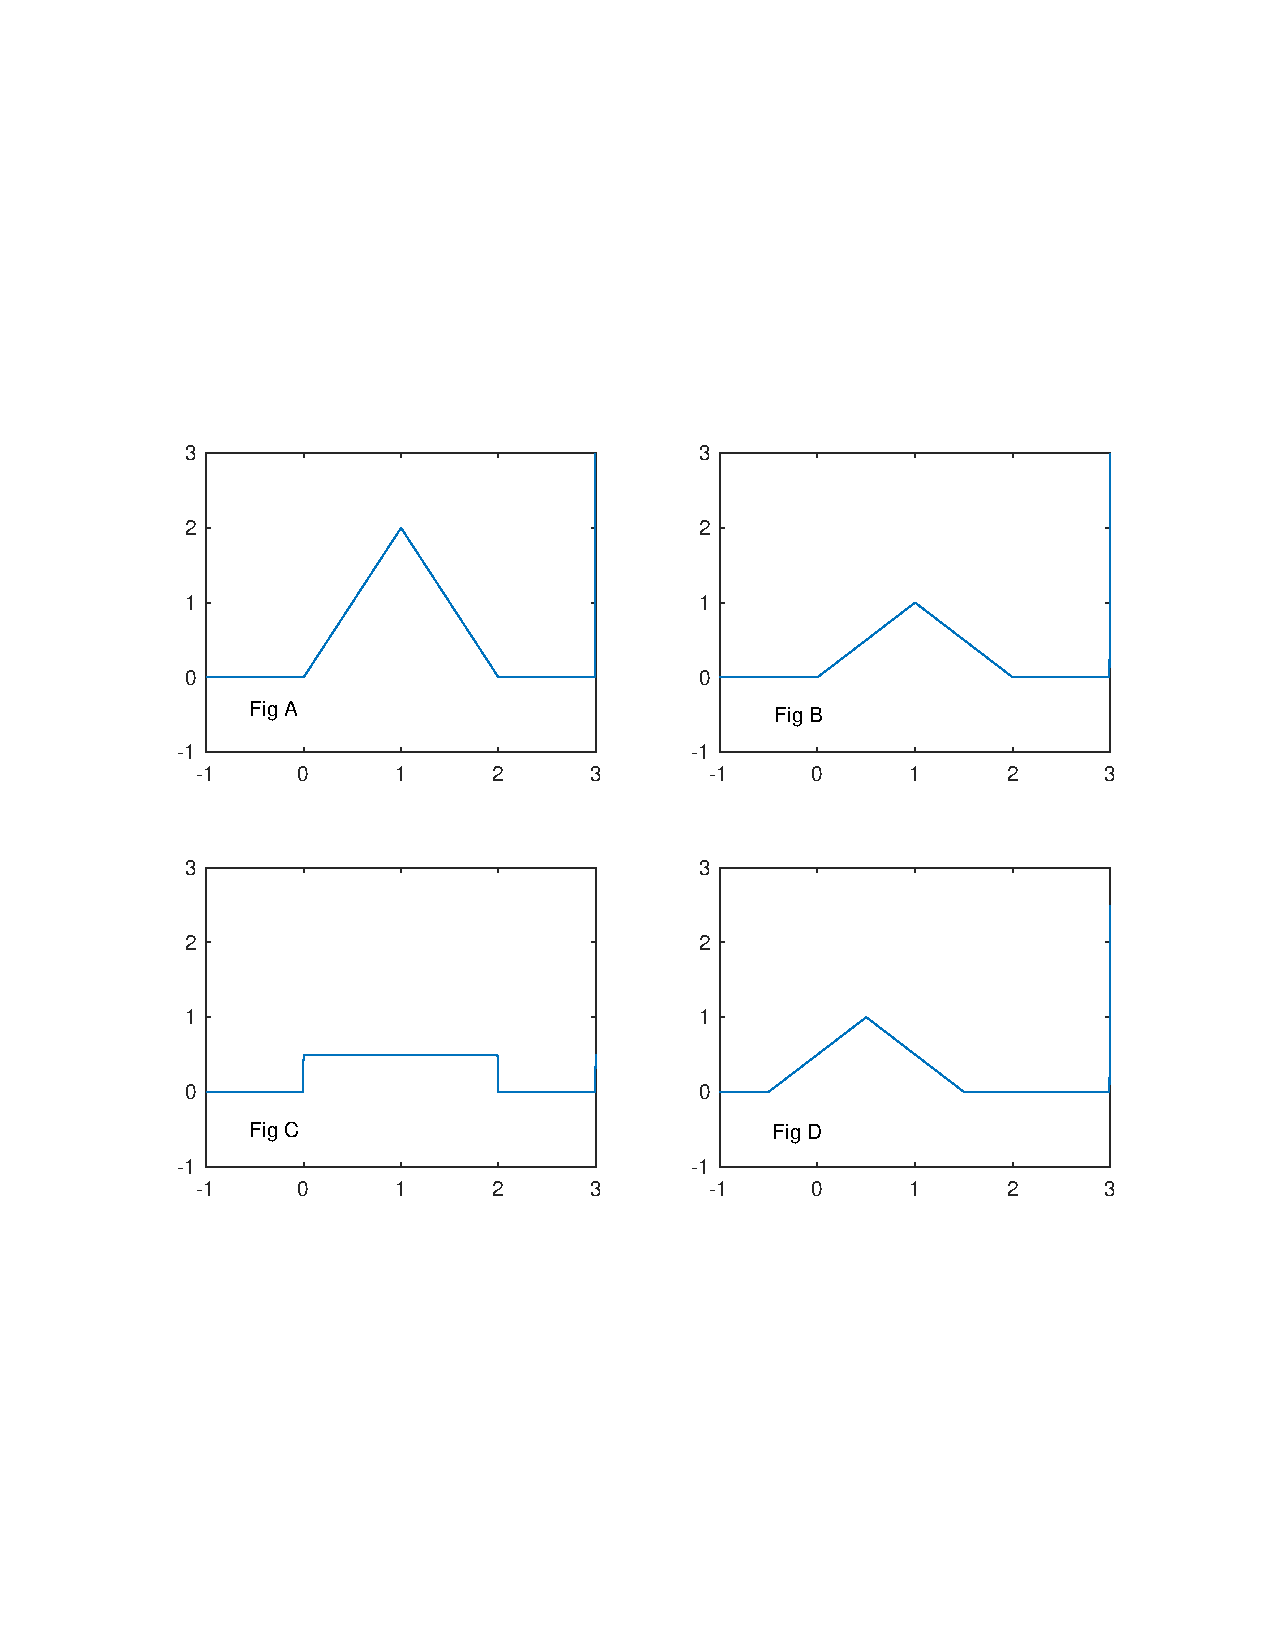
\includegraphics[scale=.5]{figures/school_work/MTH_464/HW_1/figures.pdf}
\end{figure}

\vspace{-1.4in}
\sol
Figure B is the correct answer.

\newline
Figure A is wrong because the area of the function integrates to 2. \\
Figure C is wrong because it labels all possibilities as equally likely, which is not the case. \\
Figure D is wrong because it labels values below 0 as possible, which should not be the case.


\newpage
\question
Assume $X$ is a random variable with differentiable pdf $f_X(x)$. Define the \textbf{mediam} of $X$ as the value $\nu$ such that $P(X \leq \nu) = P(X \geq \nu) = \frac{1}{2}$. Show that the minimum of $g(a) = E\paren{\abs{X - a}}$ occurs at $a = \nu$.

\begin{proof}
We wish to show that $\frac{d}{da}g(a) = 0$

$$\frac{d}{da} g(a) = E\paren{\abs{X - a}} = \frac{d}{da} \npint \abs{x - a}f_X(x)dx = \frac{d}{da}\paren{\nvint{a} (a - x)f_X(x)dx + \vpint{a} (x - a)f_X(x)dx} =$$

$$= \frac{d}{da}\paren{\nvint{a} af_X(x)dx - \nvint{a} xf_X(x)dx + \vpint{a}xf_X(x)dx - \vpint{a} af_X(x)dx} =$$

$$= \frac{d}{da}\nvint{a} af_X(x)dx - \frac{d}{da}\nvint{a} xf_X(x)dx + \frac{d}{da}\vpint{a}xf_X(x)dx - \frac{d}{da}\vpint{a} af_X(x)dx =$$

$$= \frac{d}{da}a\nvint{a} f_X(x)dx - \frac{d}{da}\nvint{a} xf_X(x)dx + \frac{d}{da}\vpint{a}xf_X(x)dx - \frac{d}{da}a\vpint{a} f_X(x)dx =$$

$$= \paren{\nvint{a} f_X(x)dx + a\frac{d}{da}\nvint{a}f_X(x)dx } - \frac{d}{da}\nvint{a} xf_X(x)dx + \frac{d}{da}\vpint{a}xf_X(x)dx - \paren{\vpint{a} f_X(x)dx + a\frac{d}{da}\vpint{a} f_X(x)dx} =$$

$$= F_X(a) + a\paren{f_X(x)}\Big|_{-\infty}^a - \paren{xf_X(x)}\Big|_{-\infty}^a + \paren{xf_X(x)}\Big|_a^\infty - \paren{1 - F(a)} - a\paren{f_X(x)}\Big|_a^\infty = $$

$$= 2F_X(a) - 1 + af_X(a) - af_X(a) - af_X(a) + af_X(a) = 2F_X(a) - 1 = 0$$

Then $F_X(a) = \frac{1}{2}$, and $g(a)$ has a critical point at $a = \nu$. It remains to be shown that $a = \nu$ is minimal.

$$\frac{d}{da} g'(a) = \frac{d}{da} \paren{2F_X(a) - 1} = 2f_X(a) > 0 \text{ for all $a \in \R$ by definition of a pdf}$$

Notice that for $\eps > 0$ and very small, $g'(\nu - \eps) = 2F_X(\nu - \eps) - 1 < 2F_X(\nu) - 1 = 0$. Thus $g'(\nu - \eps) < 0$. Observe also that $g'(\nu + \eps) = 2F_X(\nu + \eps) - 1 > 2F_X(\nu) - 1 = 0$. So $g'(\nu + \eps) > 0$.
\newline

Using both of these facts, we conclude that since $g'(\nu - \eps) < 0$ and $g'(\nu + \eps) > 0$ with $g''(\nu) > 0$, the lone critical point $a = \nu$ must be a minimum.
\end{proof}
\end{questions}

\end{document}